\begin{frame}
  \begin{center}
    The object model and the semantics of the Io language
  \end{center}
\end{frame}

\begin{frame}
  \begin{center}
    Prototype-based
  \end{center}
  \note{
    \begin{itemize}
      \item Javascript uses this, too
    \end{itemize}
  }
\end{frame}

\begin{frame}
  \begin{center}
    No class
  \end{center}
  \note{
    \begin{itemize}
      \item how do we create objects?
    \end{itemize}
  }
\end{frame}

\begin{frame}
  \begin{center}
    Cloning objects
  \end{center}
\end{frame}

\begin{frame}[fragile]
  \begin{center}
    \begin{lstlisting}
      Vehicle := Object clone
    \end{lstlisting}
  \end{center}
  \note{
    \begin{itemize}
      \item Object is provided by interpreter
    \end{itemize}
  }
\end{frame}

\begin{frame}[fragile]
  \begin{center}
    \begin{lstlisting}
      Vehicle description := "Something"
    \end{lstlisting}
  \end{center}
  \note{
    \begin{itemize}
      \item creating slots
    \end{itemize}
  }
\end{frame}

\begin{frame}[fragile]
  \begin{center}
    \begin{lstlisting}
      Vehicle description # => "Something"
    \end{lstlisting}
  \end{center}
  \note{
    \begin{itemize}
      \item we sent a message with a slot name
    \end{itemize}
  }
\end{frame}
  
\begin{frame}[fragile]
  \begin{center}
    \begin{lstlisting}
      Vehicle description = "Ble"
      Vehicle otherSlot = "Ble" # => Error
    \end{lstlisting}
    \end{center}
\end{frame}  
 
\begin{frame}[fragile]
  \begin{center}
    \begin{lstlisting}
      Vehicle slotNames 
      # => list("type", "description")
    \end{lstlisting}
  \end{center}
\end{frame}
  
\begin{frame}[fragile]
  \begin{center}
    \begin{lstlisting}
      Vehicle type # => Vehicle
    \end{lstlisting}
  \end{center}
\end{frame}

\begin{frame}[fragile]
  \begin{center}
    \begin{lstlisting}
      Object type # => Object
    \end{lstlisting}
  \end{center}
\end{frame}  

\begin{frame}[fragile]
  \begin{center}
    \begin{lstlisting}
      Car := Vehicle clone
    \end{lstlisting}
  \end{center}
\end{frame}  

\begin{frame}[fragile]
  \begin{center}
    \begin{lstlisting}
      Car slotNames # => list("type")
    \end{lstlisting}
  \end{center}
\end{frame}  

\begin{frame}[fragile]
  \begin{center}
    \begin{lstlisting}
      Car description # => "Ble"
    \end{lstlisting}
  \end{center}
\end{frame}  
  
\begin{frame}[fragile]
  \begin{center}
    \begin{lstlisting}
      Car type # => Car
    \end{lstlisting}
  \end{center}
\end{frame}  
  
\begin{frame}[fragile]
  \begin{center}
    \begin{lstlisting}
      ferrari := Car clone
    \end{lstlisting}
  \end{center}
\end{frame}

\begin{frame}[fragile]
  \begin{center}
    \begin{lstlisting}
      ferrari slotNames # => list()
    \end{lstlisting}
  \end{center}
  \note{
    \begin{itemize}
      \item convention - small letter, no type
      \item better code organization
    \end{itemize}
  }
\end{frame}  

\begin{frame}[fragile]
  \begin{center}
    \begin{lstlisting}
      ferrari type # => Car
    \end{lstlisting}
  \end{center}
\end{frame}

\begin{frame}
  \begin{center}
    Objects are collections of slots.
  \end{center}
  \note{
    \begin{itemize}
      \item if slot is not found it is sent to parent
    \end{itemize}
  }
\end{frame}  
  
\begin{frame}
  \begin{center}
    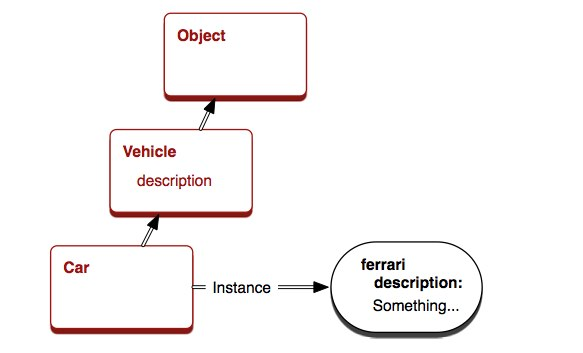
\includegraphics[width=0.8\textwidth]{images/class-based-object-model.jpg}
  \end{center}
\end{frame}

\begin{frame}
  \begin{center}
    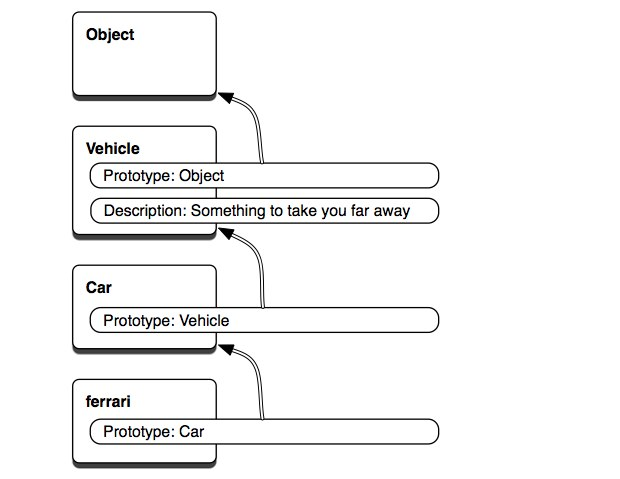
\includegraphics[width=0.8\textwidth]{images/prototype-based-object-model.jpg}
  \end{center}
\end{frame}

\begin{frame}
  \begin{center}
    Methods
  \end{center}
\end{frame}

\begin{frame}[fragile]
  \begin{center}
    \begin{lstlisting}
      method("Something" println)
    \end{lstlisting}
  \end{center}
\end{frame}

\begin{frame}[fragile]
  \begin{center}
    \begin{lstlisting}
      Car drive := method("Vroom" println)
    \end{lstlisting}
    \begin{lstlisting}
      ferrari drive # => Vroom
    \end{lstlisting}
  \end{center}
\end{frame}  
  
\begin{frame}[fragile]
  \begin{center}
    \begin{lstlisting}
      ferrari getSlot("drive") 
      # => method("Vroom" println)
    \end{lstlisting}
  \end{center}
\end{frame}  
  
\begin{frame}[fragile]
  \begin{center}
    \begin{lstlisting}
      ferrari proto # => Car
      Car proto # => Vehicle
    \end{lstlisting}
  \end{center}
\end{frame}  

\begin{frame}
  \begin{center}
    true, false, nil
  \end{center}
\end{frame}
  
\begin{frame}[fragile]
  \begin{center}
    Singletons
    \vskip15pt
    \onslide<2->
    
    \begin{lstlisting}
      MyType clone := MyType
    \end{lstlisting}
  \end{center}
  \note{
    \begin{itemize}
      \item how to create a singleton?
    \end{itemize}
  }
\end{frame}
  
\begin{frame}[fragile]
  \begin{center}
    \begin{lstlisting}
      Object clone := "dupa"
    \end{lstlisting}
  \end{center}
\end{frame}

\begin{frame}
  \begin{center}
    Messages
  \end{center}
  \note{
    \begin{itemize}
      \item all interactions are done with messages
      \item everything is a message (and message is an object)
    \end{itemize}
  }
\end{frame}  

\begin{frame}
  \begin{center}
    Message
    \begin{itemize}
      \item<2-> sender
      \item<3-> target
      \item<4-> arguments
    \end{itemize}
  \end{center}
\end{frame}

\begin{frame}[fragile]
  \begin{center}
    \begin{lstlisting}
      for(i, 1, 10, i println)
      a := if(b = = 0, c + 1, d)
    \end{lstlisting}
  \end{center}
\end{frame}

\begin{frame}
  \begin{center}
    Reflection
  \end{center}
\end{frame}
  